\documentclass{eptcs}
\usepackage{tikz}
\usepackage{wrapfig}
\usepackage{subcaption}
\usepackage{amsthm}
\usepackage{amsmath}
\usepackage{graphicx}
\usepackage{float}
\usepackage{gensymb}
\usepackage{multicol}
\usepackage{pgfplotstable} 
\usepackage{booktabs} 
\usepackage{filecontents}
\usepackage{longtable}
\usepackage{tabu}
\setlength{\columnsep}{1cm}
\usepackage{tabu} % if you want
\newtheorem{theorem}{Theorem}

\setcounter{secnumdepth}{0}
\usetikzlibrary {positioning}
\definecolor {processblue}{cmyk}{0.96,0,0,0}


\DeclareMathOperator*{\argmin}{\arg\!\min}
%\usepackage{breakurl}             % Not needed if you use pdflatex only.

\title{Fake News Classification using Machine Learning} %don't forget to change running title too!
\author{
David Anuta
\and
Patrick Ferner
\and
Som Liengtiraphan
\and
Vasim Patel
\and
Jonathan Scott
\and
Eric Weiss
}
\def\titlerunning{Fake News Classification using Machine Learning}
\def\authorrunning{}
\begin{document}
\maketitle
% |------------|
% | Abstract |
% |------------|
\begin{abstract}
	The goal of our project was to have a program that would be able to classify and identify “fake news”. Our plan was to use different methods of analysis on the articles to detect patterns in how fake news articles are written. We had many ideas and explored many different ways to analyze the articles, including lexical analysis, sentiment analysis and network analysis. As part of our final product, we implemented an SVM, and trained on data produced by a Naive Bayes Classifier and Topic Modeling. We wanted the SVM to be able to take in an article, and determine if it is real or fake. We trained our SVM on articles from Politico, Breitbart, New York Times, Wall Street Journal, and a database of peer reviewed fake articles. Our SVM resulted in being able to correctly classify an article around 90\% of the time.
\end{abstract}
\section*{Description of Problem}
In the modern age of the internet, we are constantly inundated with  more information that we can carefully analyze. This overload has led malicious groups to flood the internet with fake news. Now more than ever, the need to distinguish facts from the fiction in popular media is imperative. The objective of this project is to create a tool that can learn to label fake and real news. This will be done using machine learning techniques on a pre-labeled corpus of articles to properly learn ways to distinguish between fake and real news.
\section*{Literature Review}
Various methods for detecting fake news have previously been implemented and discussed throughout the available literature. The methods that were utilized in the development of our Fake News detector were pulled from the available literature and tested. The best or more interesting of these features/methods were used (or at least considered) in our implementation of this classifier. Below is a discussion of some of the available literature as pertaining to the topic of fake news classification and some of the useful/interesting features that we obtained from these.

\subsection*{Detecting Fake Medical Web Sites Using Recursive Trust Labeling}
In  “Detecting Fake Medical Web Sites Using Recursive Trust Labeling”, Ahmed Abbasi, Fatemeh Zahedi, and Siddharth Kaza, built an adaptive learning algorithm that would identify fake medical website. This is an important issue because fraudulent medical websites provide inaccurate and misleading medical information. Many of these websites are facades for malicious organizations whose only goal is to scam customers. Sites like these have led to severe public safety ramifications. They not only generate millions of dollars through scams, but their fictitious advice also leads to thousands of deaths. This paper thus proposes an adaptive learning algorithm they have named RTL, or recursive trust labeling to identify, and thus combat this problem. 

There are 3 types of fake medical websites: “spoof, concocted, and Web spam”. The RTL algorithm uses “underlying content and graph-based classifiers” as well as recursive labeling to enhance fake medical site detection. The content classifier also utilizes other components such as medical thesauruses to compensate for the different complexities that occur in medical literature. 

The algorithm was tested on almost 100 million links between 930,000 web sites. In that test set, 1,000 of the sites were known legitimate and fake medical sites. The test resulted in an overall accuracy of 94\%, a significant improvement in fake medical website detection over 19 other adaptive learning approaches. This high rate of  accuracy is even maintained when the training dataset is composed of as little as 30 websites. 

Previous fake website detectors had focused on “the application of content” or “graph-based detection methods...targeting end users or Web spam sites targeting search engines”. This new algorithm proposes the fusion of content and graphical analysis that adapts to new information. 

Content analyses looks at the subject matter of the website and access the word choice, presentation, and tone. Their content classification method stemmed from their observation that fake medical websites appear templatic. Speculation of this phenomenon is that “fraudsters frequently expedite the development of fake Web sites by using automatic content generation techniques to mass produce Web pages”. These similarities can then be exploited through machine learning algorithms to help detect other fake medical websites. Techniques that were utilized to learn the patterns of these patterns included support vector machines, neural networks, bayesian networks, naive bayes, C4.5, and logistic regression. 

Graph analyses looks at the structural information of a website and how it’s connects and relate to other websites. Their graph-based method stemmed from another observation that fake medical websites spend millions of dollars on search engine optimization in order to inflate the perceived importance of their website. These optimizations are done using link farms, websites that point to the fake website to increase website visibility. Thus, graph-based methods have been created to combat there link farms. They are created under the assumption that “good pages link to other good pages and bad pages link to other bad pages”.  These network analyses then assess the quality of the web page to determine the genuity of the information. Examples of other graph-based methods include PageRank, TrustRank, BadRank, Parent Penalty, Anti-TrustRank, Mass Estimation, and Cautious Surfer. 

The recursive trust labelling algorithm works by utilizing prior studies on content and graphical analyses and recursively expanding the training dataset “by selecting additional test instances during each iteration”. The goal is to have the training set revise their classification after each round of new information.

This type of graphical/network analysis was considered for our implementation. As with fake medical websites, fake news should link to (and be linked to by) other fake sources/articles. A graphical based analysis of the articles would likely increase the ability for classification of fake news. Sadly, due to time constraints and the problems associated with defining how a source or article is linked to another article, this type of graphical analysis was not used in fake news detection system.

\subsection*{A Comparison of Fraud Clues and Classification Methods for Fake Escrow Website Detection}
This article is an examination of the techniques already available and how effective they are at identifying fake auction websites. Written by  Ahmed Abbasi and Hsinchun Chen, they compare different fraud cues and classification methods, such as “support vector machines, neural networks, decision trees, naı¨ve bayes, and principal component analysis” algorithms over extracted fraud cues from web page text, images, and link information. The test set consisted of 90,000 web pages from 410 legitimate and fake auction websites. The results from this experiment were that a combination of methods produced 90\% accuracy while an ensemble of support vector machines produced 96\% accuracies when differentiating fake websites from real ones. It was also determined that to accurately identify fake websites, a broad set of fraud cues must be considered in the analysis to combat the large gamut of tactics used by fraudsters. 

It is difficult to fully alleviate fraudulent auction websites because 2 problems: “easy identity changes and reputation manipulation”. It is easy for fraudsters to change their domain and identity once they are identified as a fake site.  Reputation manipulation refers to similar SEO manipulation and link farms mentioned in the previous article that boosts the visibility of the page to appear genuine. To combat the adaptive nature of the fraud auction website industry, the study assesses the feasibility of automated systems to identify fake websites to help reduce the negative impact of online auctions. 

An assessment of the fraud cues is thus necessary to create this automated system. These fraud cues fall into 5 categories: website content, website design, URL and anchor text, images, and website linkage and structure. 

Web content for most fake auction websites are automatically generated in order to mass produce these websites. Thus, websites appear more templatic with “repetition of stylistic patterns in the page content (i.e., body text and URLs) and design (i.e., HTML) as well as duplication of images and icons”. These websites also frequently contain spelling mistakes and grammatical mistakes. Other things that were included in their classification process were “words per page, words per title, average word length, and word n-gram frequencies”.

Website design is examined through analysis of the HTML code. Elements such as font type, sizes, and colors have been used to for “stylometric categorization” through inspection of things such as tag n-grams. Since many of these fake websites have similar website designs, analysis of HTML code through SVM will be able to group similarly designed pages together. 

URL and anchor text in fraud auction websites often contained more dashes, digits, and more characters than real websites. Fake websites also tend to use the unsecured “http” instead of “https”. The number of slashes “/” indicate page levels and fake websites tend to contain deeper home pages. Fraudulent auction websites also tend to have URL suffixes that end with “.org” (as they can pose as non-profit organizations, “.biz”, or “.us”. 

Image analysis is trickier due to indexing content, making collecting and analysis more difficult. However, it was noted in their studies that many of these websites used the same images, banners, and icons. 

Lastly, linkage features provide crucial information about the credibility of a web page. The in/back links and out links can be used to create context graphs to construct a multilayer graph provides insight into the “structural signature” of different website types. A key feature of these structural identities are that fake auction websites are designed to deceive online traders, while over types of spam websites are intended to deceive search engines. This difference in audiences gives the fake auction websites a different aesthetic that is specially designed to appeal to online buyers. 

The team experiments to determine the effectiveness of various feature sets and classification techniques. First, they compared six features (body text, HTML, URL, image, link, and all) and five techniques (SVM, Winnow, C4.5, NB, and PCA). The found that the HTML, URL, and body text analysis provided a 80\% accuracy level while the image feature provided a 70\% accuracy rate, however it is enough to suggest that image duplication is common among fake auction sites. The use of all features did the best overall, with 3-5\% more accuracy than individual testing. This also suggest that all the individual feature sets provide “important complementary discriminatory potential”, they each contribute an important piece of the puzzle and a fusion of all of them is the best mode of action to classify fake auction websites.

In terms of classification algorithms, SVM had the best performance of all the techniques, producing an accuracy rate of 90\% in overall performance. Winnow, did slightly better than SVM when detecting URL features. PCA and NB did the worst performance, doing a 10-20\% lower accuracy rate. Thus, it can be concluded that the best technique to classify fake auction website would be to use SVM. 

In conclusion, the study suggest that the best plan of action to detect fake auction website is to employ a top-level SVM classifier over the whole range of fraud cue features. By utilizing this method over all the feature, the study was able to achieve an 96\% site level classification performance. Rather than testing for each feature individually, the study indicate that a fusion of all the features will improve the classification process by 2-10\%. 

The features discussed above were also discussed for our implementation of identifying fake news. The result, that SVM was the best method, is a large part of why we chose to try to implement an SVM to try to classify fake news. We did not end up using any of the above features, as we found that they seemed detrimental to our overall classification when combined with our other approaches.

\section*{Data Preparation}
To prep the data for analysis, we created a database using PostgreSQL. We started with around 300,000 articles from Breitbart and Politico. We then added articles scrapped from the New York Times and The Wall Street Journal. A dataset of articles identified as fake was also retrieved from Kaggle and added to the database. In total, our database ended up storing 333,574 articles. The tables in this database include articles, article\_tags, tags, source\_authors, authors, sources, article\_authors, and tokens. We indexed each article, author, source, and tag by id, and gave them attributes that we were interested in querying. For example, our article table contains title, url, content, etc. We also have what we call “linking tables” which relate two table rows together. These relations include linking between articles and tags, articles and authors, and sources and authors. These linking tables are mainly for storage purposes. A similar result could have be accomplished by storing a list within each row of a table which held ids corresponding to the linked items in the other, linked, table. However, the implementation of our “linking tables” bypassed this method of storage so that when writing cross table queries for linked items a user would not have to iterate across a list of ids in order to find the proper result. Though more storage intensive at large scale, we decided that this query optimization would be overall beneficial to the database. Below is a picture of the current database.
\begin{figure}[H]
	\centering
	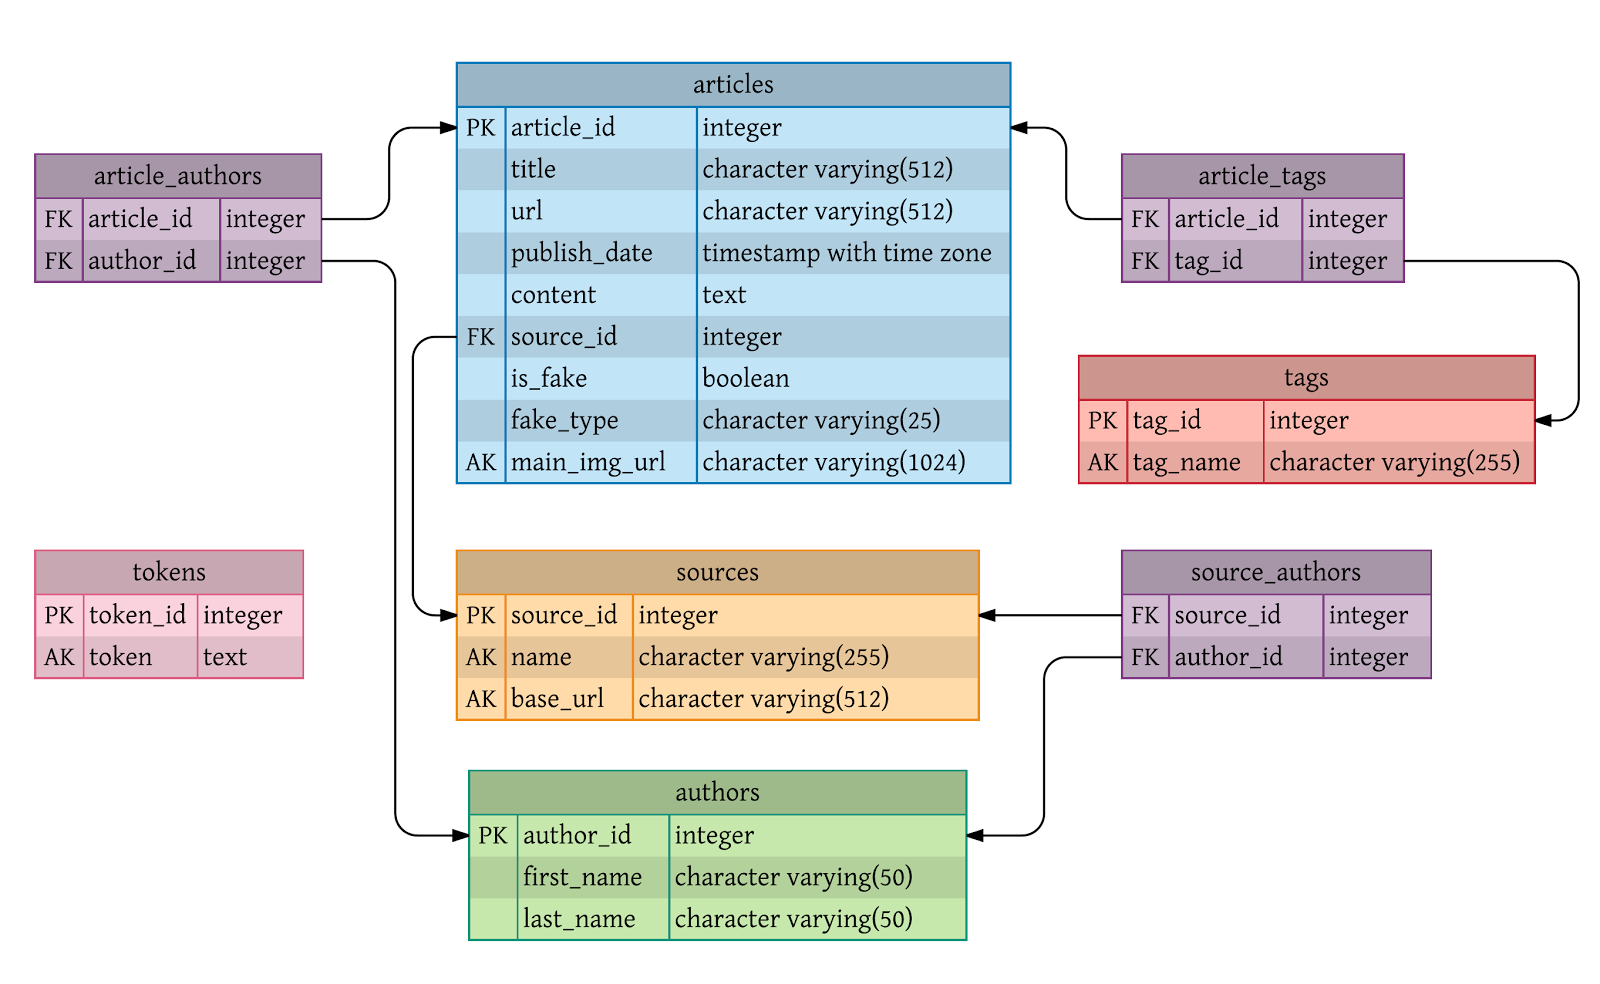
\includegraphics[scale=.3]{db_diagram}
\end{figure}

\section*{Discussion of Approach}
\subsection*{Naive Bayes Classifier}
Our first step towards fake news classification was using a bayesian network. To properly illustrate the use of a bayesian network (and to learn how to construct one) we created a simple bayesian network to identify the the news source of an article from our database. At the time of testing, the database only contained articles from BreitBart and Politico.

Using NLTK (the Natural Language Toolkit for Python), we created a dictionary based tool that has a list of scores for each word that appear in a test set. Once we have the tool that has been trained to recognize a particular pattern from one source, we experimented to see if the Bayesian classifier can correctly recognize if a random article we feed it is from Politico or Breitbart. 

\end{document}